%%%%%%%%%%%%%%%%%%% vorlage.tex %%%%%%%%%%%%%%%%%%%%%%%%%%%%%
%
% LaTeX-Vorlage zur Erstellung von Projekt-Dokumentationen
% im Fachbereich Informatik der Hochschule Trier
%
% Basis: Vorlage svmono des Springer Verlags
%
%%%%%%%%%%%%%%%%%%%%%%%%%%%%%%%%%%%%%%%%%%%%%%%%%%%%%%%%%%%%%

\documentclass[envcountsame,envcountchap, deutsch]{i-studis}

\usepackage{makeidx}         	% Index
\usepackage{multicol}        	% Zweispaltiger Index
%\usepackage[bottom]{footmisc}	% Erzeugung von Fußnoten

%%-----------------------------------------------------
%\newif\ifpdf
%\ifx\pdfoutput\undefined
%\pdffalse
%\else
%\pdfoutput=1
%\pdftrue
%\fi
%%--------------------------------------------------------
%\ifpdf
\usepackage[pdftex]{graphicx}
\usepackage{epstopdf}
\usepackage[pdftex,plainpages=false]{hyperref}
%\else
%\usepackage{graphicx}
%\usepackage[plainpages=false]{hyperref}
%\fi

%%-----------------------------------------------------
\usepackage{color}				% Farbverwaltung
%\usepackage{ngerman} 			% Neue deutsche Rechtsschreibung
\usepackage[english, ngerman]{babel}
%\usepackage[latin1]{inputenc} 	% Ermöglicht Umlaute-Darstellung
%\usepackage[utf8]{inputenc}  	% Ermöglicht Umlaute-Darstellung unter Linux (je nach verwendetem Format)
\usepackage[T1]{fontenc}
\usepackage{textcomp}

%-----------------------------------------------------
\usepackage{listings} 			% Code-Darstellung
\lstset
{
	basicstyle=\scriptsize, 	% print whole listing small
	keywordstyle=\color{blue}\bfseries,
								% underlined bold black keywords
	identifierstyle=, 			% nothing happens
	commentstyle=\color{red}, 	% white comments
	stringstyle=\ttfamily, 		% typewriter type for strings
	showstringspaces=false, 	% no special string spaces
	framexleftmargin=7mm, 
	tabsize=3,
	showtabs=false,
	frame=single, 
	rulesepcolor=\color{blue},
	numbers=left,
	linewidth=146mm,
	xleftmargin=8mm
}
\usepackage{textcomp} 			% Celsius-Darstellung
\usepackage{amssymb,amsfonts,amstext,amsmath}	% Mathematische Symbole
\usepackage[german, ruled, vlined]{algorithm2e}
\usepackage[a4paper]{geometry} % Andere Formatierung
\usepackage{bibgerm}
\usepackage{array}
\hyphenation{Ele-men-tar-ob-jek-te  ab-ge-tas-tet Aus-wer-tung House-holder-Matrix Le-ast-Squa-res-Al-go-ri-th-men} 		% Weitere Silbentrennung bei Bedarf angeben
\setlength{\textheight}{1.1\textheight}
\pagestyle{myheadings} 			% Erzeugt selbstdefinierte Kopfzeile
\makeindex 						% Index-Erstellung


%--------------------------------------------------------------------------
\begin{document}
%------------------------- Titelblatt -------------------------------------
\title{Funktionsprinzipien und Anwendungen von Algorithmen zur Pfadplanung}
\project{Ausarbeitung zur Vorlesung Wissenschaftliches Arbeiten}
%--------------------------------------------------------------------------
\supervisor{Titel Vorname Name} 		% Betreuer der Arbeit
\author{Bearbeiter 1: Mohammed Salih Mezraoui \\Bearbeiter 2: David Gruber \\Bearbeiter 3: Marius Müller}							% Autor der Arbeit
\groupid{WissArb22/Thema 2/Gruppe-7}
\address{Trier,} 							% Im Zusammenhang mit dem Datum wird hinter dem Ort ein Komma angegeben
\submitdate{15.07.2022} 				% Abgabedatum
%\begingroup
%  \renewcommand{\thepage}{title}
%  \mytitlepage
%  \newpage
%\endgroup
\begingroup
  \renewcommand{\thepage}{Titel}
  \mytitlepage
  \newpage
\endgroup
%--------------------------------------------------------------------------
\frontmatter 
%--------------------------------------------------------------------------
\kurzfassung

%% deutsch
\paragraph*{}
In dieser wissenschaftlichen Arbeit werden Algorithmen zur Pfadplanung dargestellt und analysiert. Es wird anhand der Anwendung in Geoinformationssystemen und bei mobilen Robotern aufgezeigt, wie der Algorithmus von Dijkstra eingesetzt wird und welche Stärken und Schwächen damit einhergehen.  Da die Fragestellungen, die mit Algorithmen zur Pfadplanung bearbeitet werden, immer komplexer werden, steigen auch die Anforderungen an Zeit- und Platzkomplexität. Daher werden in dieser Arbeit die wichtigsten Optimierungsstrategien für Algorithmen zur Pfadplanung dargestellt. In einer experimentellen Analyse konnte gezeigt werden, dass die Laufzeit des Algorithmus von Dijkstra durch den Einsatz von Preprocessing und heuristischer Funktionen um mehrere Größenordnungen gesenkt werden kann. 


 			% Kurzfassung Deutsch/English
\tableofcontents 						% Inhaltsverzeichnis
%--------------------------------------------------------------------------
\mainmatter                        		% Hauptteil (ab hier arab. Seitenzahlen)
%--------------------------------------------------------------------------
% Die Kapitel werden in separaten .tex-Dateien abgelegt und hier eingebunden.
\chapter{Einleitung und Problemstellung}

Begonnen werden soll mit einer Einleitung zum Thema, also Hintergrund und Ziel erläutert werden.

Weiterhin wird das vorliegende Problem diskutiert: Was ist zu lösen, warum ist es wichtig, dass man dieses Problem löst und welche Lösungsansätze gibt es bereits. Der Bezug auf vorhandene oder eben bisher fehlende Lösungen begründet auch die Intention und Bedeutung dieser Arbeit. Dies können allgemeine Gesichtspunkte sein: Man liefert einen Beitrag für ein generelles Problem oder man hat eine spezielle Systemumgebung oder ein spezielles Produkt (z.B. in einem Unternehmen), woraus sich dieses noch zu lösende Problem ergibt.

Im weiteren Verlauf wird die Problemstellung konkret dargestellt: Was ist spezifisch zu lösen? Welche Randbedingungen sind gegeben und was ist die Zielsetzung? Letztere soll das
beschreiben, was man mit dieser Arbeit (mindestens) erreichen möchte.
\chapter{Weitere Kapitel}

Die Gliederung hängt natürlich vom Thema und von der Lösungsstrategie ab. Als nützliche
Anhaltspunkte können die Entwicklungsstufen oder - schritte z.B. der Softwareentwicklung betrachtet werden. Nützliche Gesichtspunkte erhält und erkennt man, wenn man sich
\begin{itemize}
  \item in die Rolle des Lesers oder
  \item in die Rolle des Entwicklers, der die Arbeit z.B. fortsetzen, ergänzen oder pflegen soll,
\end{itemize}
versetzt. In der Regel wird vorausgesetzt, dass die Leser einen fachlichen Hintergrund haben - z.B. Informatik studiert haben. D.h. nur in besonderen, abgesprochenen Fällen schreibt man in populärer Sprache, so dass auch Nicht-Fachleute die Ausarbeitung prinzipiell lesen und verstehen können.

Die äußere Gestaltung der Ausarbeitung hinsichtlich Abschnittformate, Abbildungen, mathematische Formeln usw. wird in \hyperref[Stile]{Kapitel~\ref*{Stile}} kurz dargestellt.
\chapter{LaTeX-Bausteine}\label{Stile}

Der Text wird in bis zu drei Ebenen gegliedert:

\begin{enumerate}
  \item Kapitel ( = chapter),
  \item Unterkapitel/Abschnitte  ( = section) 
  \item Unterunterkapitel/Unterabschnitte  ( = subsection).
\end{enumerate}

\section{Abschnitt}\index{Abschnitt}
Text der Gliederungsebene 2.


\subsection{Unterabschnitt} \index{Unterabschnitt}
Text der Gliederungsebene 3.
Text Text Text Text Text Text Text Text Text Text Text Text Text Text Text
Beispiel für Quelltext\index{Quelltext} \\[2 ex]
\noindent
\begin{minipage}{1.0\textwidth} \small
\begin{lstlisting}
	Prozess 1:
	
	Acquire();
		a := 1;
	Release();
	...
	Acquire();
	if(b == 0)
	{					
		c := 3;
		d := a;
	}				
	Release();
\end{lstlisting}
\end{minipage}

\vspace{2cm}
\noindent
\begin{minipage}{1.0\textwidth} \small
\begin{lstlisting}
	Prozess 2:
	
	Acquire();
		b := 1;
	Release();
	...
	Acquire();
	if(a == 0)
	{					
		c := 5;
		d := b;
	}				
	Release();
\end{lstlisting}
\end{minipage}
\vskip 1em

Größere Code-Fragmente sollten im Anhang eingefügt werden.

\section{Abbildungen und Tabellen}

Abbildung\index{Abbildung} und Tabellen\index{Tabelle} werden zentriert eingefügt. Grundsätzlich sollen sie
erst dann erscheinen, nach dem sie im Text angesprochen wurden (siehe Abb. \ref{a1}). Abbildungen und Tabellen (siehe Tabelle \ref{t1}) können
im (fließenden) Text (= here ), am Seitenanfang (= top ), am Seitenende
(= bottom ) oder auch gesammelt auf einer nachfolgenden Seite (= page )
oder auch ganz am Ende der Ausarbeitung erscheinen. Letzteres sollte man nur
dann wählen, wenn die Bilder günstig zusammen zu betrachten sind und die
Ausarbeitung nicht zu lang ist ($< 20$ Seiten).

\begin{figure} %[hbtp]
	\centering
		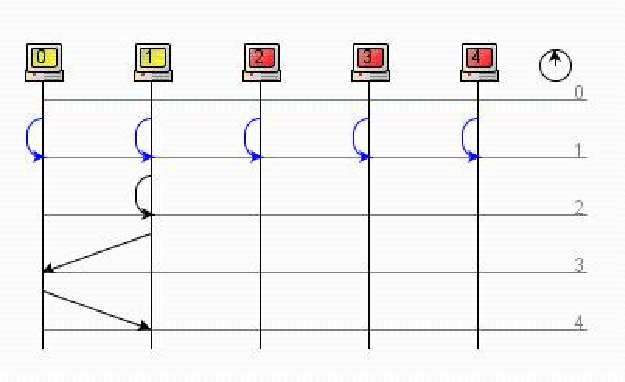
\includegraphics{images/p1ReadSeq.pdf}
	\caption{Bezeichnung der Abbildung}
	\label{a1}
\end{figure}

\begin{table} %[hbtp]
	\centering
		\begin{tabular}{l | l l l l}
		\textbf{Prozesse} & \textbf{Zeit} $\rightarrow$ \\
		\hline
			$P_{1}$ & $W(x)1$ \\
			$P_{2}$ & & $W(x)2$ \\
			$P_{3}$ & & $R(x)2$ & & $R(x)1$\\
			$P_{4}$ & & & $R(x)2$ & $R(x)1$\\
		\end{tabular}
	\caption{Bezeichnung der Tabelle}
	\label{t1}
\end{table}


\section{Mathematische Formel}\index{Formel}
Mathematische Formeln bzw. Formulierungen können sowohl im
laufenden Text (z.B. $y=x^2$) oder abgesetzt und zentriert im Text
erscheinen. Gleichungen sollten für Referenzierungen nummeriert
werden (siehe Formel \ref{gl-1}).
\begin{equation}
\label{gl-1}
e_{i}=\sum _{i=1}^{n}w_{i}x_{i}
\end{equation}

Entscheidungsformel:

\begin{equation}
\psi(t)=\left\{\begin{array}{ccc}
1 &  \qquad 0 <= t < \frac{1}{2} \\
-1 &  \qquad \frac{1}{2} <= t <1 \\
0 & \qquad sonst
\end{array} \right.
\end{equation}


Matrix:\index{Matrix}
\begin{equation}
A = \left(
\begin{array}{llll}
a_{11} & a_{12} & \ldots & a_{1n} \\
a_{21} & a_{22} & \ldots & a_{2n} \\
\vdots & \vdots & \ddots & \vdots \\
a_{n1} & a_{n2} & \ldots & a_{nn} \\
\end{array}
\right)
\end{equation}

Vektor:\index{Vektor} 

\begin{equation}
\overline{a} = \left(
\begin{array}{c}
a_{1}\\
a_{2}\\
\vdots\\
a_{n}\\
\end{array}
\right)
\end{equation}

\section{Sätze, Lemmas und Definitionen}\index{Satz}\index{Lemma}\index{Definition}

Sätze, Lemmas, Definitionen, Beweise,\index{Beweis} Beispiele\index{Beispiel} können in speziell dafür vorgesehenen Umgebungen erstellt werden.

\begin{definition}(Optimierungsproblem)

Ein \emph{Optimierungsproblem} $\mathcal{P}$ ist festgelegt durch ein Tupel
$(I_\mathcal{P}, sol_\mathcal{P}, m_\mathcal{P}, goal)$ wobei gilt

\begin{enumerate}
\item $I_\mathcal{P}$ ist die Menge der Instanzen,
\item $sol_\mathcal{P} : I_\mathcal{P} \longmapsto \mathbb{P}(S_\mathcal{P})$ ist eine Funktion, die jeder Instanz $x \in I_\mathcal{P}$ eine Menge zulässiger Lösungen zuweist,
\item $m_\mathcal{P} : I_\mathcal{P} \times S_\mathcal{P} \longmapsto \mathbb{N}$ ist eine Funktion, die jedem Paar $(x,y(x))$ mit $x \in I_\mathcal{P}$ und $y(x) \in sol_\mathcal{P}(x)$ eine
Zahl $m_\mathcal{P}(x,y(x)) \in \mathbb{N}$ zuordnet (= Maß für die Lösung $y(x)$ der Instanz $x$), und
\item $goal \in \{min,max\}$.
\end{enumerate}

\end{definition}

\begin{example} MINIMUM TRAVELING SALESMAN (MIN-TSP)
\begin{itemize}
\item $I_{MIN-TSP} =_{def}$ s.o., ebenso $S_{MIN-TSP}$
\item $sol_{MIN-TSP}(m,D) =_{def} S_{MIN-TSP} \cap \mathbb{N}^m$ 
\item $m_{MIN-TSP}((m,D),(c_1, \ldots , c_m)) =_{def} \sum_{i=1}^{m-1} D(c_i, c_{i+1}) + D(c_m,c_1)$ 
\item $goal_{MIN-TSP} =_{def} min$
\end{itemize}
\begin{flushright}
$\qed$
\end{flushright}
\end{example}

\begin{theorem} Sei $\mathcal{P}$ ein \textbf{NP}-hartes Optimierungsproblem.
Wenn $\mathcal{P} \in$ \textbf{PO}, dann ist \textbf{P} = \textbf{NP}.
\end{theorem}

\begin{proof} Um zu zeigen, dass \textbf{P} = \textbf{NP} gilt, genügt es
wegen Satz A.30 zu zeigen, dass ein einziges \textbf{NP}-vollständiges
Problem in \textbf{P} liegt. Sei also $\mathcal{P}'$ ein beliebiges \textbf{NP}-vollständiges Problem.

Weil $\mathcal{P}$ nach Voraussetzung \textbf{NP}-hart ist, gilt insbesondere
$\mathcal{P}' \leq_T \mathcal{P}_C$. Sei $R$ der zugehörige
Polynomialzeit-Algorithmus dieser Turing-Reduktion.
Weiter ist $\mathcal{P} \in$ \textbf{PO} vorausgesetzt, etwa vermöge eines
Polynomialzeit-Algorithmus $A$. Aus den beiden
Polynomialzeit-Algorithmen $R$ und $A$ erhält man nun
leicht einen effizienten Algorithmus für $\mathcal{P}'$: Ersetzt man
in $R$ das Orakel durch $A$, ergibt dies insgesamt eine polynomielle
Laufzeit. 
%\begin{flushright}
$\qed$
% \end{flushright}
\end{proof}

\begin{lemma} Aus \textbf{PO} $=$ \textbf{NPO} folgt \textbf{P} $=$ \textbf{NP}.
\end{lemma}

\begin{proof} Es genügt zu zeigen, dass unter der angegeben
Voraussetzung KNAPSACK $\in$ \textbf{P} ist.

Nach Voraussetung ist MAXIMUM KNAPSACK $\in$ \textbf{PO},
d.h. die Berechnung von $m^*(x)$ für jede Instanz $x$ ist
in Polynomialzeit möglich. Um KNAPSACK bei Eingabe
$(x,k)$ zu entscheiden, müssen wir nur noch $m^*(x) \geq k$
prüfen. Ist das der Fall, geben wir $1$, sonst $0$ aus. Dies
bleibt insgesamt ein Polynomialzeit-Algorithmus. 
\begin{flushright}
$\qed$
\end{flushright}
\end{proof}

\section{Fußnoten}

In einer Fußnote können ergänzende Informationen\footnote{Informationen die für die Arbeit zweitrangig sind, jedoch für den Leser interessant sein könnten.} angegeben werden. Außerdem kann eine Fußnote auch Links enthalten. Wird in der Arbeit eine Software (zum Beispiel Java-API\footnote{\url{http://java.sun.com/}}) eingesetzt, so kann die Quelle, die diese Software zur Verfügung stellt in der Fußnote angegeben werden.

\section{Literaturverweise}\index{Literatur}
Alle benutzte Literatur wird im Literaturverzeichnis angegeben\footnote{Dazu wird ein sogennanter bib-File, literatur.bib verwendet.}. Alle angegebene Literatur sollte mindestens einmal im Text referenziert werden\cite{Coulouris:02}.
\chapter{Beispiel-Kapitel}

In diesem Kapitel wird beschrieben, warum es unterschiedliche Konsistenzmodelle\index{Konsistenzmodelle} gibt. Außerdem werden die Unterschiede zwischen strengen Konsistenzmodellen\index{Linearisierbarkeit} (Linearisierbarkeit, sequentielle Konsistenz)\index{sequentiell!Konsistenz} und schwachen Konsistenzmodellen\index{Konsistenz!schwach} (schwache Konsistenz, Freigabekonsistenz)\index{Freigabekonsistenz} erläutert. Es wird geklärt, was Strenge und Kosten (billig, teuer) in Zusammenhang mit Konsistenzmodellen bedeuten.

\section{Warum existieren unterschiedliche Konsistenzmodelle?}

Laut \cite{Malte:97} sind mit der\index{Replikation} Replikation von Daten immer zwei gegensätzliche Ziele verbunden: die Erhöhung der\index{Verfügbarkeit} Verfügbarkeit und die Sicherung der\index{Konsistenz} Konsistenz der Daten. Die Form der Konsistenzsicherung bestimmt dabei, inwiefern das eine Kriterium erfüllt und das andere dementsprechend nicht erfüllt ist (Trade-off zwischen Verfügbarkeit und der Konsistenz der Daten). Stark konsistente Daten sind stabil, das heißt, falls mehrere Kopien der Daten existieren, dürfen keine Abweichungen auftreten. Die Verfügbarkeit der Daten ist hier jedoch stark eingeschränkt. Je schwächer die Konsistenz wird, desto mehr Abweichungen können zwischen verschiedenen Kopien einer Datei auftreten, wobei die Konsistenz nur an bestimmten Synchronisationspunkten gewährleistet wird. Dafür steigt aber die Verfügbarkeit der Daten, weil sie sich leichter replizieren lassen.

Nach \cite{Mosberger:93} kann die Performanzsteigerung der schwächeren Konsistenzmodelle wegen der Optimierung\index{Optimierung} (Pufferung, Code-Scheduling, Pipelines) 10-40 Prozent betragen. Wenn man bedenkt, dass mit der Nutzung der vorhandenen Synchronisierungsmechanismen schwächere Konsistenzmodelle den Anforderungen der strengen Konsistenz genügen, stellt sich der höhere programmiertechnischer Aufwand bei der Implementierung der schwächeren Konsistenzmodelle als ihr einziges Manko dar.

In \cite{Cheriton:85} ist beschrieben, wie man sich Formen von DSM vorstellen könnte, für die ein beachtliches Maß an\index{Inkonsistenz} Inkonsistenz akzeptabel wäre. Beispielsweise könnte DSM verwendet werden, um die Auslastung von Computern in einem Netzwerk zu speichern, so dass Clients für die Ausführung ihrer Applikationen die am wenigsten ausgelasteten Computer auswählen können. Weil die Informationen dieser Art innerhalb kürzester Zeit ungenau werden können (und durch die Verwendung der veralteten Daten keine großen Nachteile entstehen können), wäre es vergebliche Mühe, sie ständig für alle Computer im System konsistent zu halten \cite{Coulouris:02}. Die meisten Applikationen stellen jedoch strengere Konsistenzanforderungen.

\section{Klassifizierung eines Konsistenzmodells}

Die zentrale Frage, die für die Klassifizierung\index{streng}\index{schwach} (streng oder schwach) eines Konsistenzmodells von Bedeutung ist \cite{Coulouris:02}: wenn ein Lesezugriff auf eine Speicherposition erfolgt, welche Werte von Schreibzugriffen auf diese Position sollen dann dem Lesevorgang bereitgestellt werden? Die Antwort für das schwächste Konsistenzmodell lautet: von jedem Schreibvorgang, der vor dem Lesen erfolgt ist, oder in der "`nahen"' Zukunft, innerhalb des definierten Betrachtungsraums, erfolgten wird. Also irgendein Wert, der vor oder nach dem Lesen geschrieben wurde.

Für das strengste Konsistenzmodell, Linearisierbarkeit (atomic consistency), stehen alle geschriebenen Werte allen Prozessoren sofort zur Verfügung: eine Lese-Operation gibt den aktuellsten Wert zurück, der geschrieben wurde, bevor das Lesen stattfand. Diese Definition ist aber in zweierlei Hinsicht problematisch. Erstens treten weder Schreib- noch Lese-Operationen zu genau einem Zeitpunkt auf, deshalb ist die Bedeutung von "`aktuellsten"' nicht immer klar. Zweitens ist es nicht immer möglich, genau festzustellen, ob ein Ereignis vor einem anderen stattgefunden hat, da es Begrenzungen dafür gibt, wie genau Uhren in einem verteilten System synchronisiert werden können.

Nachfolgend werden einige Konsistenzmodelle absteigend nach ihrer Strenge vorgestellt. Zuvor müssen wir allerdings klären, wie die Lese- und Schreibe-Operationen in dieser Ausarbeitung dargestellt werden.

Sei $x$ eine Speicherposition, dann können Instanzen dieser Operationen wie folgt ausgedrückt werden:
\begin{itemize}
	\item $R(x)a$ - eine Lese-Operation\index{Operation!Lese}, die den Wert $a$ von der Position $x$ liest.
	\item $W(x)b$ - eine Schreib-Operation\index{Operation!Schreib}, die den Wert $b$ an der Position $x$ speichert.
\end{itemize}

\section{Linearisierbarkeit\index{Linearisierbarkeit} (atomic consistency)}

Die Linearisierbarkeit im Zusammenhang mit DSM kann wie folgt definiert werden:
\begin{itemize}
	\item Die verzahnte Operationsabfolge findet so statt: wenn $R(x)a$ in der Folge vorkommt, dann ist die letzte Schreib-Operation, die vor ihr in der verzahnten Abfolge auftritt, $W(x)a$, oder es tritt keine Schreib-Operation vor ihr auf und $a$ ist der Anfangswert von $x$. Das bedeutet, dass eine Variable nur durch eine Schreib-Operation geändert werden kann.
	\item Die Reihenfolge der Operationen in der Verzahnung ist konsistent zu den \underline{Echtzeiten}\index{Echtzeiten}, zu denen die Operationen bei der tatsächlichen Ausführung aufgetreten sind.
\end{itemize}

Die Bedeutung dieser Definition kann an folgendem Beispiel (Tabelle \ref{tab:1}) nachvollzogen werden. Es sei angenommen, dass alle Werte mit $0$ vorinitialisiert sind.

\begin{table}
	\centering
		\begin{tabular}{l | l l l l}
			\textbf{Prozesse} & \textbf{Zeit} $\rightarrow$ & \\
			\hline
			$P_{1}$ & $W(x)1$ & & $W(y)2$ \\
			$P_{2}$ & & $R(x)1$ & & $R(y)2$ \\
		\end{tabular}
	\caption{Linearisierbarkeit ist erfällt}
	\label{tab:1}
\end{table}

Hier sind beide Bedingungen erfüllt, da die Lese-Operationen den zuletzt geschriebenen Wert zurückliefern. Interessanter ist es, zu sehen, wann die Linearisierbarkeit verletzt ist.

\begin{table}
	\centering
		\begin{tabular}{l | l l l l}
		\textbf{Prozesse} & \textbf{Zeit} $\rightarrow$ \\
		\hline
		$P_{1}$ & $W(x)1$ & $W(x)2$ \\
		$P_{2}$ & & & \color{red} $R(x)0$ & \color{black} $R(x)2$ \\
		\end{tabular}
	\caption{Linearisierbarkeit ist verletzt, sequentielle Konsistenz ist erfüllt.}
	\label{tab:2}
\end{table}

In diesem Beispiel (Tabelle \ref{tab:2}) ist die Echtzeit-Anforderung verletzt, da der Prozess $P_{2}$ immer noch den alten Wert liest, obwohl er von Prozess $P_{1}$ bereits geändert wurde. Diese Ausführung wäre aber sequentiell konsistent (siehe kommender Abschnitt), da es eine Verzahnung der Operationen gibt, die diese Werte liefern könnte ($R(x)0$, $W(x)1$, $W(x)2$, $R(y)2$). Würde man beide Lese-Operationen des 2. Prozesses vertauschen, wie in der Tabelle \ref{tab:3} dargestellt, so wäre keine sinnvolle Verzahnung mehr möglich.

\begin{table}
	\centering
		\begin{tabular}{l | l l l l}
		\textbf{Prozesse} & \textbf{Zeit} $\rightarrow$ \\
		\hline
		$P_{1}$ & $W(x)1$ & $W(x)2$ \\
		$P_{2}$ & & & \color{red} $R(x)2$ &  \color{red} $R(x)0$ \\
			
		\end{tabular}
	\caption{Linearisierbarkeit und sequentielle Konsistenz sind verletzt.}
	\label{tab:3}
\end{table}

In diesem Beispiel sind beide Bedingungen verletzt. Selbst wenn die Echtzeit, zu der die Operationen stattgefunden haben, ignoriert wird, gibt es keine Verzahnung einzelner Operationen, die der Definition entsprechen würde.
\chapter{Zusammenfassung und Ausblick}
\label{Zusammenfassung und Ausblick}
In den letzten Jahren hat die Pfadplanung immer mehr an Relevanz gewonnen, zum Beispiel wird beim autonomen Autofahren immer mehr Forschung 
im Bereich der Pfadplanungsalgorithmen betrieben \cite{Karur:21}.
\noindent \\
\begin{itemize}
    \item Bevor ein Programm mit der Suche nach der besten Lösung (dem besten Weg) beginnen kann, muss erst ein Ziel deklariert und das Problem (Umgebung) genau definiert werden \cite[108,109]{Russell:10}.
    \item Suchalgorithmen betrachten Zustände und Aktionen atomar, das heißt sie berücksichtigen keine interne Struktur, die sie besitzen könnten \cite[108,109]{Russell:10}.
    \item Sie werden nach folgenden Kriterien bewertet: Optimalität, Vollständigkeit, sowie Raum- und Zeitkomplexität \cite[80]{Russell:10}.
    \item Uninformierte Pfadsuchalgorithmen verfügen nur über eine grundlegende Problemdefinition und keine weiteren Metriken/Heuristiken. In dieser wissenschaftlichen Arbeit wurden folgende uninformierte Algorithmen vorgestellt:
    \begin{itemize}
        \item Die Breitensuche (Kapitel \ref{Breitensuche}) expandiert zuerst die flachsten Knoten. Sie ist vollständig, optimal für einheitliche Pfadkosten, hat jedoch eine exponentielle Raumkomplexität \cite[81]{Russell:10}.
        \item Die Tiefensuche (Kapitel \ref{Tiefensuche}) expandiert zuerst den tiefsten nicht expandierten Knoten. Sie ist weder vollständig noch optimal, hat aber eine lineare Raumkomplexität \cite[85,86]{Russell:10}.
        \item Die iterative Vertiefungssuche (Kapitel \ref{Tiefensuche}) ist eine Wiederholung der Tiefensuche mit zunehmender Tiefenbegrenzung, bis ein Ziel gefunden wird. Sie ist vollständig, optimal für die Kosten pro Schritt, hat eine vergleichbare Zeitkomplexität wie die Breitensuche und eine lineare Raumkomplexität \cite[85,86]{Russell:10}.
        \item Der Greedy Dijkstra-Algorithmus (Kapitel \ref{Dijkstra-Algorithmus}) der zwar bei der blinden Suche Zeit vergeudet, aber dafür optimal ist und eine Trefferquote von 100\% hat \cite{Karur:21}.
        \item Die Optimierung durch eine bidirektionale Suche kann die Zeitkomplexität reduzieren, allerdings ist sie nicht immer für das Problem geeignet und kann viel Speicherplatz beanspruchen \cite[108,109]{Russell:10}.\\\\
    \end{itemize}
    \newpage
    \item Informierte Suchmethoden basieren auf heuristischen Funktionen, die die Kosten einer Lösung schätzen können \cite[108,109]{Russell:10}. 
    \begin{itemize}
        \item Der Greedy Best-First-Search-Algorithmus (Kapitel \ref{Optimierungsstrategien}) expandiert Knoten nach einem minimalen heuristischen Funktionswert. Er ist nicht optimal, aber dafür effizient \cite[108,109]{Russell:10}.
        \item A*-Suche (Kapitel \ref{A*}) expandiert Knoten mit minimalem Heuristischen Funktions- und Pfadkostenwerten. A* ist vollständig und optimal, vorausgesetzt die heuristische Funktion ist zulässig.
        \item ALT-Algorithmen (Kapitel \ref{ALT-Algorithmen}), die aufgebaut auf A* durch Preprocessing noch optimiertere Ergebnisse erzeugt.
        \item Reach-based Pruning (Kapitel \ref{Reach-Based Pruning}), welches den Dijkstra-Algorithmus um eine Metrik erweitert und dadurch optimiert.
    \end{itemize}
    \item Wie ein, durch eine heuristische Funktion optimierter, informierter Pfadsuchalgorithmus leistungsbezogen abschneidet, hängt von der Qualität der heuristischen Funktion ab \cite[108,109]{Russell:10}.
\end{itemize}

% ...
%--------------------------------------------------------------------------
\backmatter                        		% Anhang
%-------------------------------------------------------------------------
\bibliographystyle{geralpha}			% Literaturverzeichnis
\bibliography{literatur}     			% BibTeX-File literatur.bib
%--------------------------------------------------------------------------
\printindex 							% Index (optional)
%--------------------------------------------------------------------------
\begin{appendix}						% Anhänge sind i.d.R. optional
   \chapter{Glossar}

\abbreviation{ALT}{A* search, Landmarks und Triangle inequality}
\abbreviation{NP}{nichtdeterministisches, polynomialzeitliches}
% \abbreviation{DisASTer}		{DisASTer (Distributed Algorithms Simulation Terrain), A platform for the Implementation of Distributed Algorithms}
% \abbreviation{DSM}			{Distributed Shared Memory}
% \abbreviation{AC}			{Linearisierbarkeit (atomic consistency)}
% \abbreviation{SC}			{Sequentielle Konsistenz (sequential consistency)}
% \abbreviation{WC}			{Schwache Konsistenz (weak consistency)}
% \abbreviation{RC}			{Freigabekonsistenz (release consistency)}
			% Glossar   
   \chapter*{Arbeitsverteilung}

\textbf{Teilnehmer 1: Mohammed Salih Mezraoui} 
\\
 Inhalte:
 \begin{itemize}
    \item Kapitel \ref{Was ist Pfadplanung?}: Was ist Pfadplanung?
    \item Kapitel \ref{Dijkstra Algorithmus}: Dijkstra Algorithmus
    \item Kapitel \ref{Bellman-Ford-Algorithmus}: Bellman-Ford-Algorithmus
    \item Kapitel \ref{GIS(Geoinformationssystem)}: GIS(Geoinformationssystem)
    \item Kapitel \ref{Mobile Roboter}: Mobile Roboter
\end{itemize}
\paragraph*{}
\textbf{Teilnehmer 2: David Gruber} 
\\
Inhalte: 
\begin{itemize}
    \item Kapitel \ref{Einleitung und Problemstellung}: Einleitung und Problemstellung
    \item Kapitel \ref{Uninformierter Ansatz}: Uninformierter Ansatz
    \item Kapitel \ref{Autonome Navigation}: Autonome Navigation
    \item Kapitel \ref{Zusammenfassung und Ausblick}: Zusammenfassung und Ausblick
\end{itemize}
\paragraph*{}
\textbf{Teilnehmer 3: Marius Müller} 
\\
 Inhalte: 
\begin{itemize}
	\item Kapitel \ref{Optimierungsstrategien}: Optimierungsstrategien
\end{itemize}		% Welcher Studierende hat welche Texte formuliert?
   
\end{appendix}

\end{document}
